\PassOptionsToPackage{usenames,dvipsnames}{xcolor}
\documentclass[14pt]{standalone}
\usepackage{fontspec}
\usepackage{etex}
\usepackage{relsize}
\usepackage{graphicx}
\defaultfontfeatures{Mapping=tex-text}
\setmainfont[Ligatures={NoCommon, NoDiscretionary, NoHistoric, NoRequired, NoContextual}, Mapping=tex-text]{Cambria}
\usepackage{tikz,tikz-qtree}
	\usetikzlibrary{fit,backgrounds,positioning,arrows,shapes}
	\usetikzlibrary{decorations.pathreplacing}
    \tikzset{every leaf node/.style={font=\bfseries}}
\usepackage{ulem,soul}
\usepackage{array, multirow, arydshln}
\usepackage{xcolor}
	\definecolor{CB1}{RGB}{0,114,178}%BLUE
	\definecolor{CB2}{RGB}{213,94,0}%VERMILLION
	\definecolor{CB3}{RGB}{0,158,115}%BLUE GREEN
	\definecolor{CB4}{RGB}{204,121,167}%REDDISH PURPLE
	\definecolor{CB5}{RGB}{86,180,233}%SKY BLUE
	\definecolor{CB6}{RGB}{230,159,0}%ORANGE
	\definecolor{CB7}{RGB}{240,228,66}%YELLOW
	\def\CB#1#2{\textcolor{CB#1}{#2}}

\frenchspacing

\begin{document}
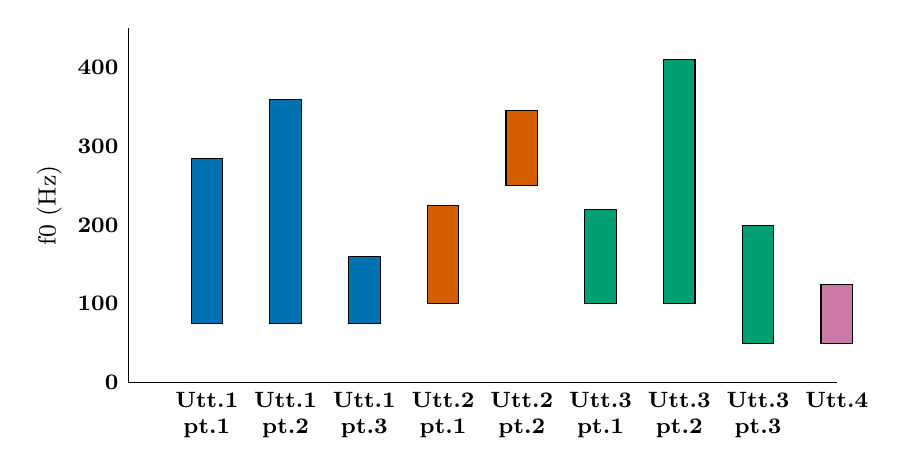
\begin{tikzpicture}
\draw (0,4.5) -- (0,0) -- (9,0);
\node[rotate=90] at (-1,2.25) {\relsize{-.5}f0 (Hz)};
\begin{scope}[anchor=east, style={font=\relsize{-1}\bfseries}]
	\node at (0,0) {0};
	\node at (0,1) {100};
	\node at (0,2) {200};
	\node at (0,3) {300};
	\node at (0,4) {400};
\end{scope}
\begin{scope}[anchor=north,align=center, style={font=\relsize{-1}\bfseries}]
	\node at (1,0) {Utt.1\\pt.1};
	\node at (2,0) {Utt.1\\pt.2};
	\node at (3,0) {Utt.1\\pt.3};
	\node at (4,0) {Utt.2\\pt.1};
	\node at (5,0) {Utt.2\\pt.2};
	\node at (6,0) {Utt.3\\pt.1};
	\node at (7,0) {Utt.3\\pt.2};
	\node at (8,0) {Utt.3\\pt.3};
	\node at (9,0) {Utt.4};
\end{scope}
\draw[fill=CB1] (.8,.75) rectangle (1.2,2.85);
\draw[fill=CB1] (1.8,.75) rectangle (2.2,3.6);
\draw[fill=CB1] (2.8,.75) rectangle (3.2,1.6);
%
\draw[fill=CB2] (3.8,1) rectangle (4.2,2.25);
\draw[fill=CB2] (4.8,2.5) rectangle (5.2,3.45);
%
\draw[fill=CB3] (5.8,1) rectangle (6.2,2.2);
\draw[fill=CB3] (6.8,1) rectangle (7.2,4.1);
\draw[fill=CB3] (7.8,.5) rectangle (8.2,2);
%
\draw[fill=CB4] (8.8,.5) rectangle (9.2,1.25);
\end{tikzpicture}

\end{document}

gs -sDEVICE=pngalpha -o ranges-bars.png -r600 ranges-bars.pdf